%%
% TUM Corporate Design LaTeX Templates
% Based on the templates from https://www.tum.de/cd
%
% Feel free to join development on
% https://gitlab.lrz.de/tum-templates/templates
% and/or to create an issue in case of trouble.
%
% tum-presentation class for scientific talks, thesis presentations, ...
%
%%

%\documentclass[4to3]{tum-presentation}
%\documentclass[navsym]{tum-presentation}
%\documentclass[nothreeliner]{tum-presentation}
%\documentclass[handout,4on1]{tum-presentation}
%\documentclass[handout,2on1]{tum-presentation}
%\documentclass[handout]{tum-presentation}
\documentclass{tum-presentation}

\addbibresource{literature.bib}

\title[Shortened Title]{Clustering-Based Sentiment Analysis for Media Agenda Setting}
\subtitle{Opinion Lab Group 2.3}
\author{Wing Sheung Leung, Qiaoxi Liu}
%\institute[]{\inst{1} Department of Electrical and Computer Engineering,
%  Technical University of Munich (TUM)\\
%  \inst{2} Department of Informatics, Technical University of Munich (TUM)}
%\date{International Conference on Mostly Scientific Topics}

\footline{\insertshortauthor~| \inserttitle}

\begin{document}

\begin{frame}[noframenumbering]
  \titlepage
\end{frame}
\begin{frame}
  \frametitle{Milestones}
  \vspace{2cm}
 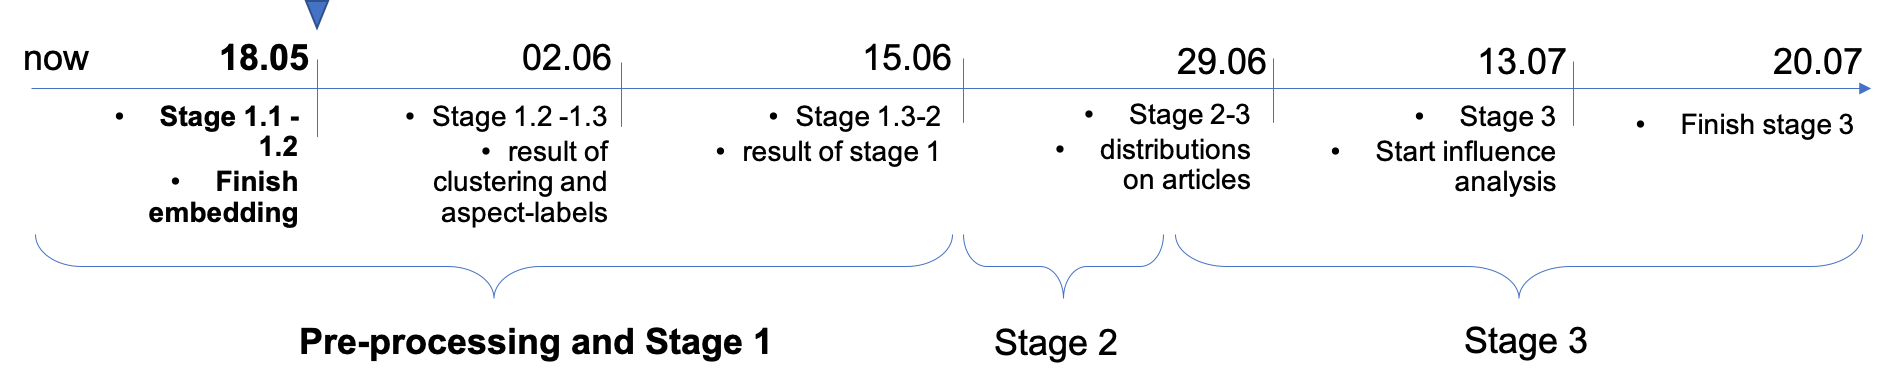
\includegraphics[width = \textwidth]{figures/timeline.png}
  
\end{frame}
\begin{frame}[t]
  \frametitle{Overview}
  \tableofcontents[sectionstyle=show,subsectionstyle=show,subsubsectionstyle=shaded]
\end{frame}



\section{Stage 1: Generate sentence embeddings with our corpus}
\subsection{1.1 Embeddings}
\subsubsection{XLING sentence-level embeddings}
\begin{frame}[fragile]
  \frametitle{Stage 1.1: XLING sentence-level embeddings}
  \begin{description}
    \item Our encoder:
  \begin{lstlisting}
  en_de_embed = hub.Module("https://tfhub.dev/google/universal-sentence-encoder-xling/en-de/1")
  \end{lstlisting}
\end{description}
  \begin{figure}[!t]
    \centering
        \begin{tabular}{cc}
            \begin{minipage}[!t]{3in}
              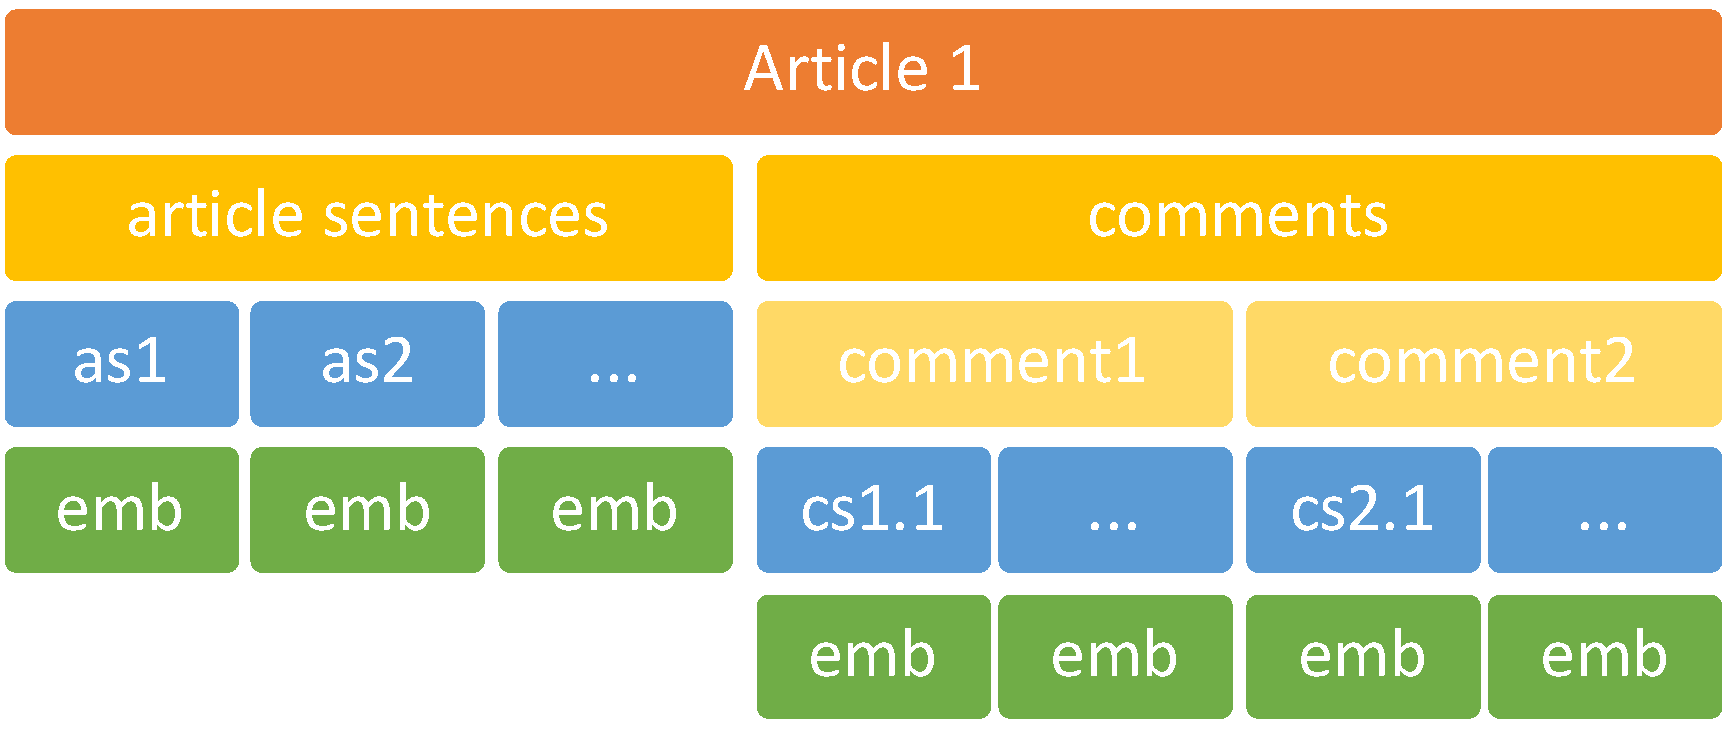
\includegraphics[width = \textwidth]{figures/hirachy.pdf}
            \caption{hierarchy of json}
            \end{minipage}
          
            \begin{minipage}[!t]{4.5in}
              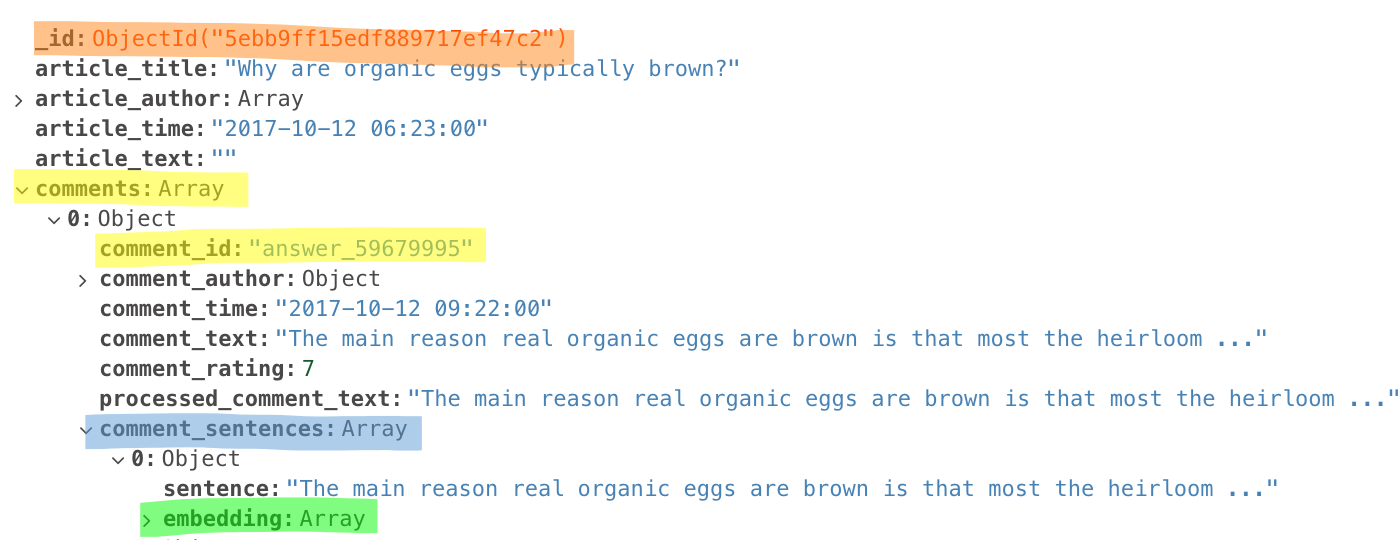
\includegraphics[width = \textwidth]{figures/example1.png}
            \caption{example from one article in quora}
            \end{minipage}
       
        \end{tabular}
    \end{figure}
  
  
\end{frame}
\subsubsection{Indexing sentences}
\begin{frame}
  
  \frametitle{Stage 1.1: Reorganize sentences from articles }
  \large
  \begin{description}
    \item Extract embeddings from nested dict to get three separate files:
    \begin{enumerate}[(i)]
      \item  embedding vectors $\to$ do clustering
      \item  strings $\to$ after clustering to generate word list, helping for define aspect labels
      \item  indexes $\to$ after sentence labeling, to do article (comments) level statistic
      \end{enumerate}
    \begin{figure}[t]
    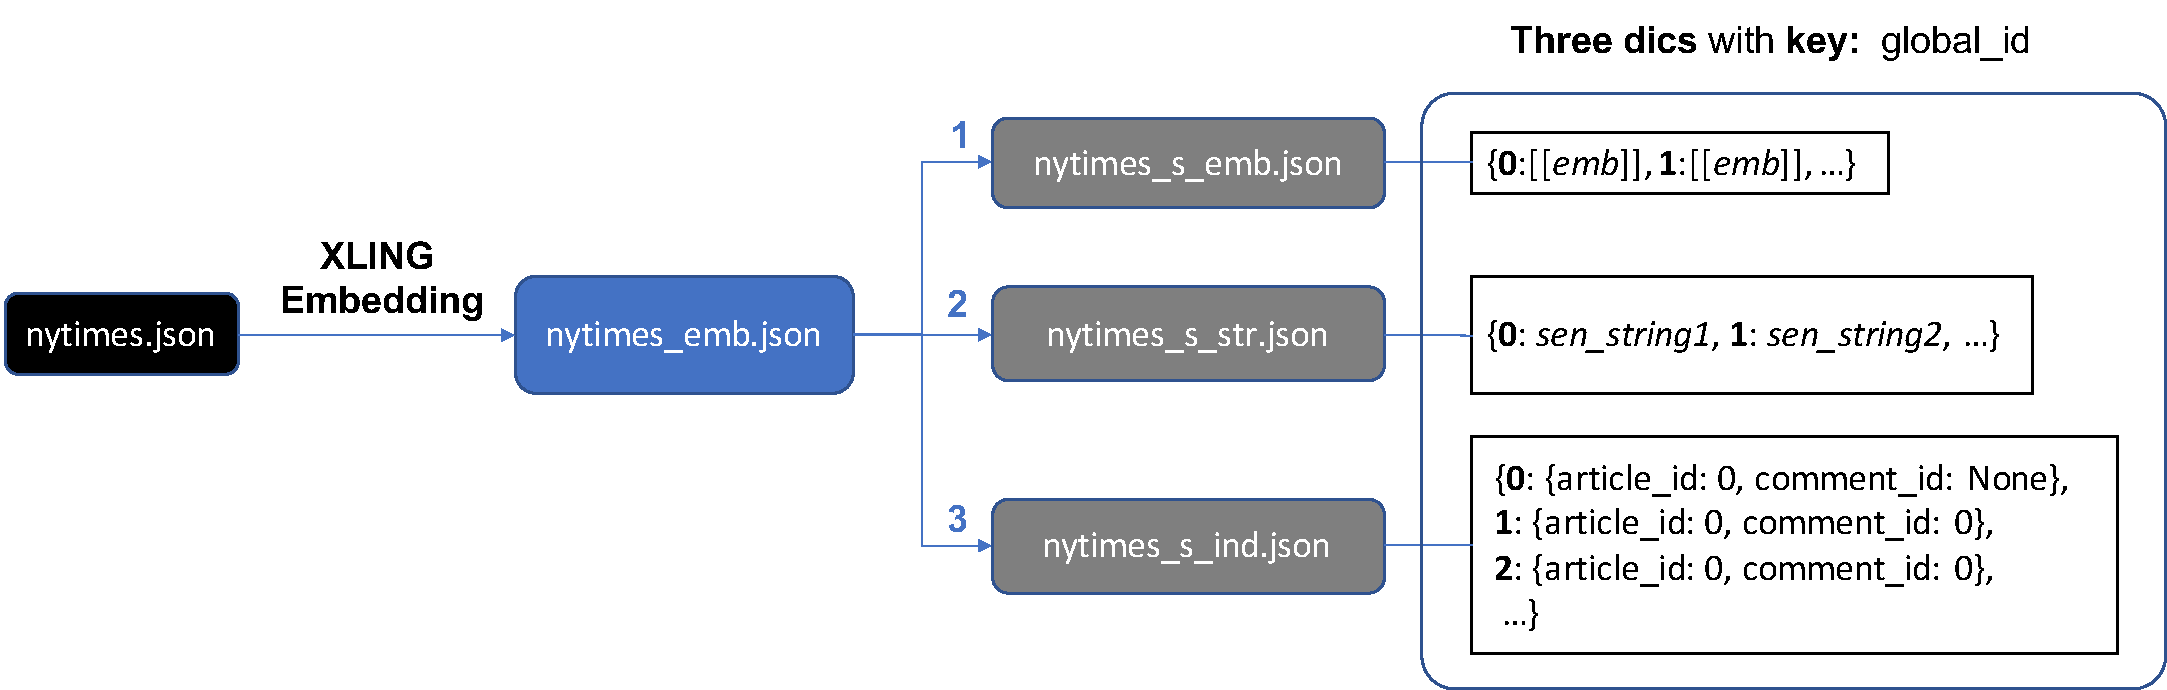
\includegraphics[width = 0.8\textwidth]{figures/diagram.pdf}
    \end{figure}
  \end{description}
\end{frame}



\subsection{1.2 Kmeans and Elbow Method}
\subsubsection{sklearn.cluster.MiniBatchKMeans}
\begin{frame}[fragile]
  \frametitle{Stage 1.2: sklearn.cluster.MiniBatchKMeans}
  \begin{lstlisting}
class KMeansClustering():
def __init__(self, k, X, is_mini_batch = True, plot_bar_chart = True):
  self.k = k
  self.X = np.array(X).reshape(len(X), 512)
  self.km = MiniBatchKMeans(n_clusters=k, init='k-means++', batch_size=3000, compute_labels=True).fit(self.X)
  \end{lstlisting}
  \begin{center}
    \begin{figure}[t]
      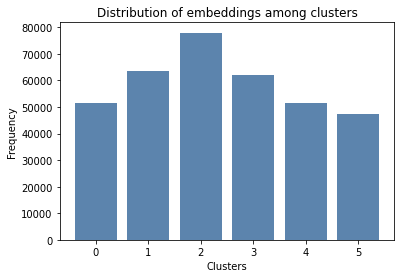
\includegraphics[width=0.35\textwidth]{images/6ks-overall-bar.png}
      \hspace{2cm}
      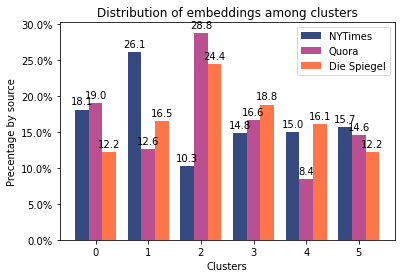
\includegraphics[width=0.35\textwidth]{images/6ks-grouped-bar.png}
      \caption{Example of distribution of embeddings of all tokenized sentences from the three sources among 6 clusters}
    \end{figure}
  \end{center}
\end{frame}
\begin{frame}[fragile]
  \frametitle{Stage 1.2: sklearn.cluster.MiniBatchKMeans}
  \framesubtitle{Why MiniBatchKmeans instead of original sklearn.cluster.KMeans}
  \begin{description}
  XLING sentence level embeddings is generated in 512 dimensions for each tokenized sentence by NLTK.
  \end{description}
  \begin{figure}[t]
    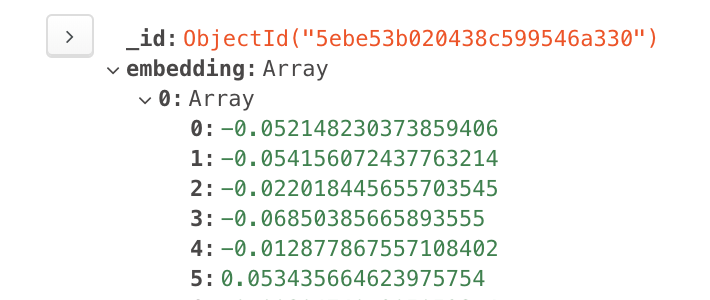
\includegraphics[width=0.35\textwidth]{presentation_2/images/embedding-sample-1.png}
    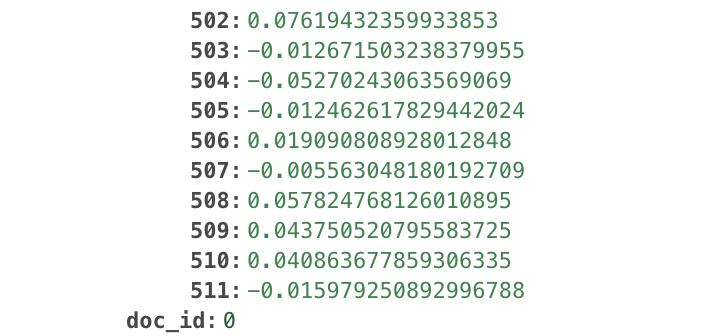
\includegraphics[width=0.35\textwidth]{presentation_2/images/embedding-sample-2.png}
    \caption{XLING embedding output for a sample sentence. Left: First 6 dimensions. Right: Last 10 dimensions}
  \end{figure}
  \small
  \begin{table}[t]
    \begin{tabular}{lcc}
    \hline
      Source & Embedding JSON size & Original corpus size\\ \hline
      New York Times & 827 MB & 55.9 MB\\
      Quora & 638 MB & 15.9 MB\\
      Die Speigel & 2.3 GB & 131 MB\\
    \hline
    \end{tabular}
    \caption{Embeddings generated are greatly larger then the original corpus size}
  \end{table}
\end{frame}
\begin{frame}[fragile]
  \frametitle{Stage 1.2: sklearn.cluster.MiniBatchKMeans}
  \framesubtitle{Why MiniBatchKmeans instead of original sklearn.cluster.KMeans}
  \begin{description}
    Just loading all sentence embeddings in Google Colaboratory, 6.36 GB out of the given 12.72 GB RAM had already been used up. 
  \end{description}
  \begin{description}
    MiniBatchKMeans is faster and helps to prevent the session from crushing, however, gives slightly different results.
  \end{description}
  \begin{figure}[t]
    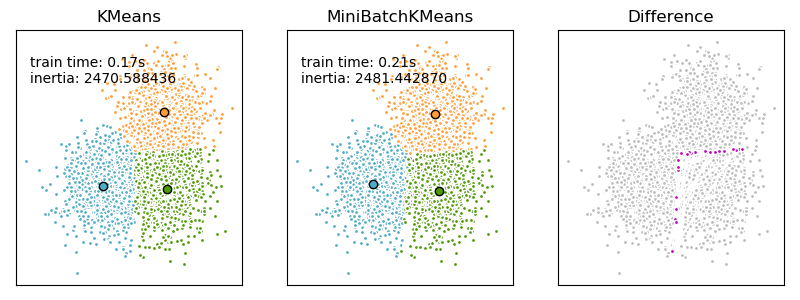
\includegraphics[width=0.60\textwidth]{images/sphx_glr_plot_mini_batch_kmeans_001.png}
    \caption{Extracted from scikit-learn; Data points classified differently are shown as purple points in 'Difference' block}
    \url{https://scikit-learn.org/stable/auto_examples/cluster/plot_mini_batch_kmeans.html}
  \end{figure}
\end{frame}
\subsubsection{Elbow Method for determining optimal k}
\begin{frame}[fragile]
  \frametitle{Stage 1.2: Elbow Method for determining optimal k}
  \begin{lstlisting}
K = range(2, 21)
for k in K:
  model = KMeansClustering(k, X)
  distortions.append(model.km.inertia_)
  \end{lstlisting}
  \begin{center}
    \begin{figure}[t]
      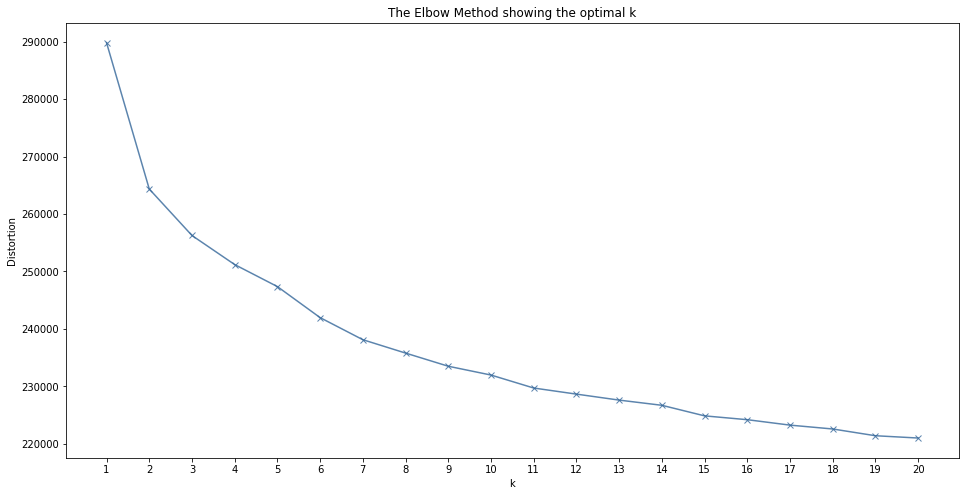
\includegraphics[width=0.5\textwidth]{images/elbow-1to20ks.png}
      \caption{No distinguishable elbow of the curve for determination of optimal k}
    \end{figure}
  \end{center}
\end{frame}

\section{Future Plan}


\begin{frame}
  \frametitle{Future Plan}
  
    
    
    \begin{figure}[t]
    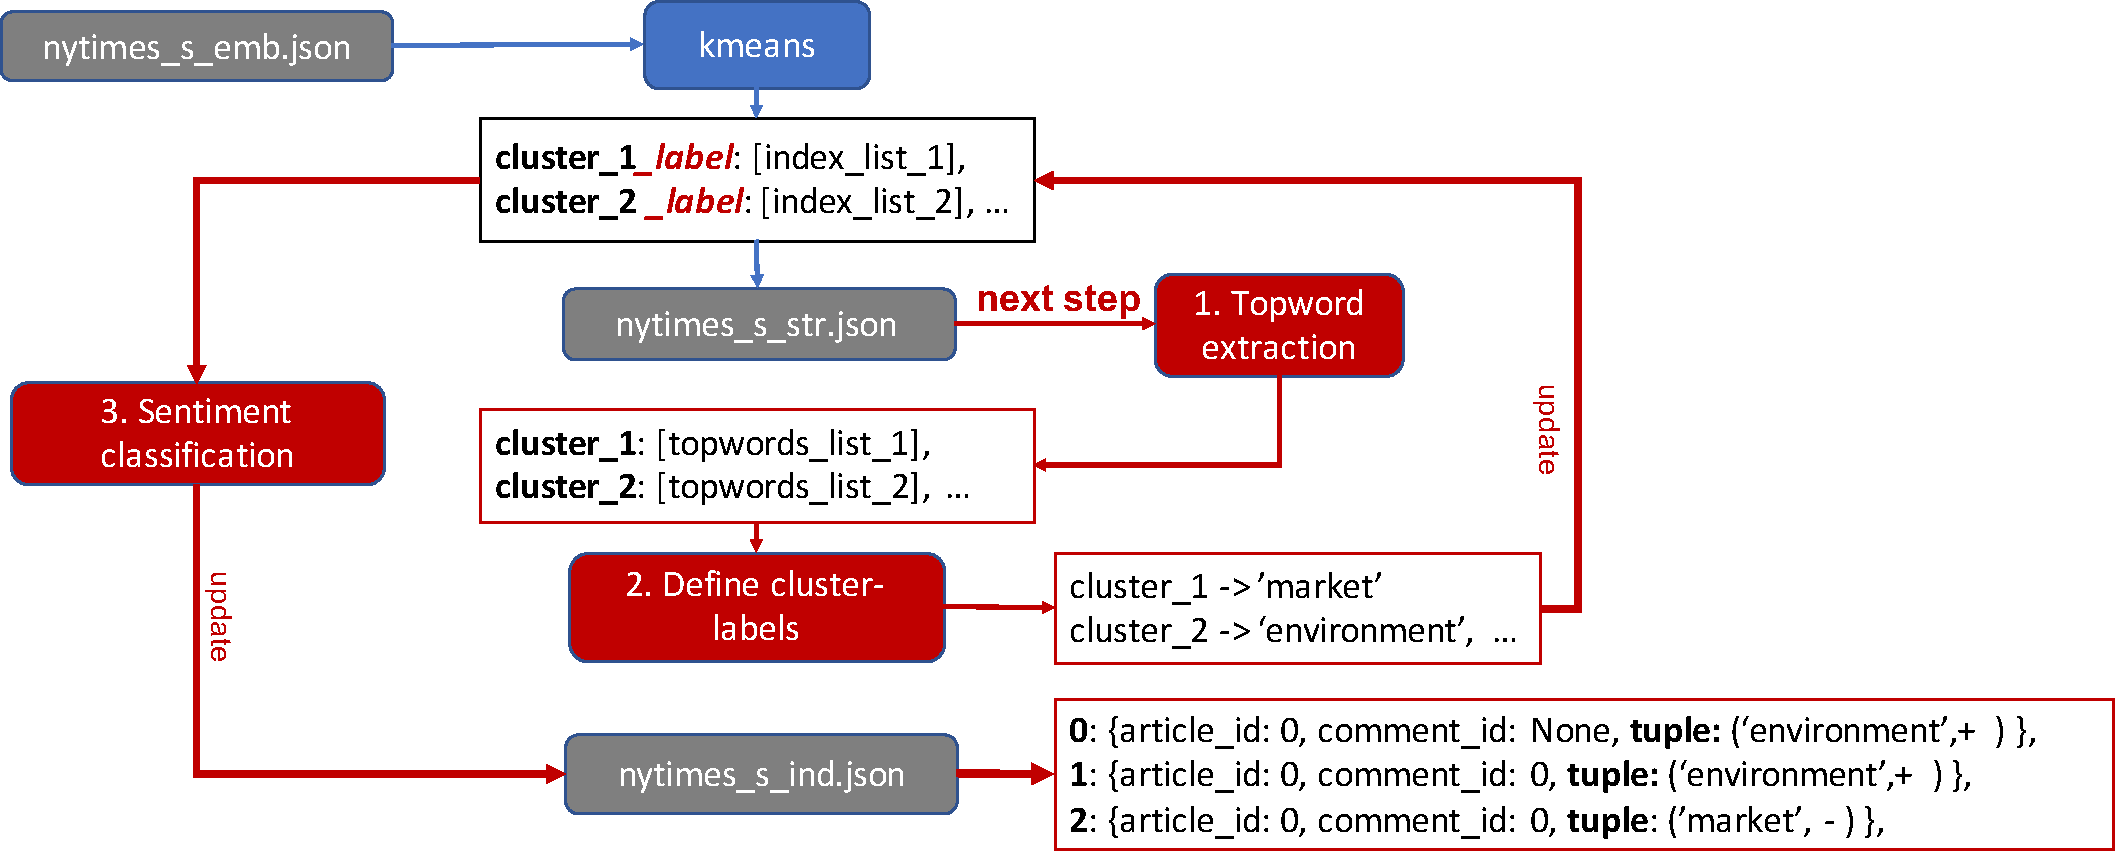
\includegraphics[width = 0.9\textwidth]{figures/plan.pdf}
    \end{figure}
 
\end{frame}

\end{document}
